%%
%% 第二章
%% 2012.5.20


\chapter{基于局部特征的图像重建算法概述}

图像重建可以被概括的定义为这样一个基本问题:从一个退化版本的二维物体估算实际的二维物体\cite{Demoment:1989tw}。退化过程的数学形式取决于图像重建算法实际的应用场景。

\section{传统的图像重建算法}
传统的图像图像重建算法所使用的场景一般是指图像修复(Image Restoration),原始“物体”由于经历了某种退化过程,不能直接由观测信息判断出来,为了消除退化过程的影响,必须根据观测到的数据进行重建来还原得到原始信息。
在图像修复中,引起退化的原因叫做失真,其定义如下:
\begin{equation}
y = A(X) \bullet b
\end{equation}
其中\(A(\cdot)\)是退化函数,可以看做是一个滤波器,b表示的是噪声,\(\bullet\)表示的叠加方式。失真通常包含对X的卷积或者模糊,加性噪声或者乘性噪声。
而图像修复的解决方案是通过对观测信息进行退化模型的数学建模,利用约束条件来推导出退化过程的逆过程,对观测信息进行逆过程得到原始图像。

另一类图像重建场景是超分辨率重建,在近年来得到飞速的发展,是炙手可热的研究领域,它的基本思想是通过多张连续的低分辨率图像序列得到一张高分辨率的图像。很多数字图像应用中都需要高分辨率的图像,高分辨率的图像能够提供更佳的视觉体验,提供更丰富的信息,比如高分辨率的医学图像能够让医生更好的进行病情诊断,高分辨率的卫星图像能够进行更准确的模式识别任务。从1970年代以来,CCD和CMOS传感器被大规模的使用,获得了大量的数字图像,但是很多图像的分辨率较低,不能满足日益增长的业务需求,超分辨率重建是在这样的背景下诞生的\cite{Park:2003hg}。

那么,我们如何通过多张低分辨率图像获得一个高分辨率图像呢?如果一个场景下有多张低分辨率图像,而且这些图像从不同的角度来“描述”这个场景,那么这些低分辨率的图像可以看做是该场景的子采样和子像素精度的位移。如果这些低分辨率图像是以整数像素为单位进行的位移,那么多张低分辨率图像没有提供任何“新的信息”,但是如果位移单位是子像素单位的,序列中的每一个图像不能够由其他图像得出,换言之每个图像都提供了子像素精度的不同信息,我们可以利用这些信息重建一个高分辨率的图像。
一般来说,SRR算法分为基于重建和基于学习的两大类:基于重建的算法如频域重建法利用图像序列的交叠关系,凸集投影(POCS)等利用一些先验知识来约束求解过程,以达到增加细节信息的目的;基于学习的算法则使用多种机器学习的概率模型,包括基于流形学习、基于支持向量机和基于独立分量的超分辨率重建技术。基于学习的方法采用大量的高分辨率图像构造学习库来训练学习模型,在对低分辨率图像进行重建的过程中引入由学习模型获得的先验知识,进而得到图像的高频细节,获得较好的图像重建效果。

总体而言,超分辨率重建的整个流程包括三个基本环节:
(1)低分辨图像的预处理,包括降噪和裁剪等基本图像数据处理。
(2)配准过程,利用像素的空间信息估算低分辨率序列图像之间的运动矢量和空间位置关系。
(3)完成重建,使用图像分割和融合等技术,利用多帧低分辨率图像的信息完成超分辨率重建。

\section{基于局部特征的图像重建算法}
从另一个角度来看,本文所采用的图像重建的部分流程可以看成是多幅图像的全景图拼接问题。与文献\cite{Brown:2006ir}中的流程类似,主要包含以下几个环节:(1)使用具有不变性的特征来描述图像;(2)自动的找到图像之间的空间位置关系,进行图像配准;(3)图像融合,消除不同图像之间的光照差别,去除边缘噪声。与全景图拼接不同的是,本文提出的图像重建系统每幅小图(Patch)块大小不一,导致图像空间位置关系可能存在不准确,多幅图像之间有大量重叠,整体思路是先融合大块,后融合小块,分别介绍如下。

\section{图像的局部特征}

\subsection{局部特征概述}
图像的局部特征是计算机视觉领域一个基本问题,它能够反映图像某一局部的特性,对寻找图像对应的局部单元以及特征描述中有着重要作用。通常意义的局部特征包含两个方面,特征检测子(Detector)和特征描述子(Descriptor)。检测子能够检测出我们“感兴趣”的点或者局部区域,而一个好的局部特征描述子反映出图像的局部特性能够帮助找到图像与图像点集合对应关系,进而建立图像之间的空间对应关系。局部图像特征描述的核心问题是不变性(invariant)和可区分性(discrimination)。

目前人们提出的众多图像局部特征中算子中,由Lowe提出的尺度不变特征变换(Scale Invariant Feature Transform,简称SIFT)应用最为广泛。1999年首次提出,至2004年得到完善\cite{Lowe:2004uq}的sift算子是图像局部特征研究领域的一项重大突破。sift算子具有很强的可区分性,同时对尺度、旋转以及一定视角和光照变化等图像变化都具有不变性。在其之上衍生出来的SURF(Speeded Up Robust Features)是对SIFT的改进版本,它利用Haar小波来近似SIFT方法中的梯度操作,同时利用积分图技术进行快速计算,SURF的速度是SIFT的3-7倍。

除此以外,常见的特征检测子包括Harris角点,ANMS等,描述子还包括DAISY,ASIFT,MROGH,BRIEF等,分别适用于不同的图像应用场景下,本文提出的系统采用适用性最广泛的sift算子,下面我们对其进行简要的介绍。

\subsection{SIFT}

(1)尺度空间理论
尺度空间理论目的是模拟图像数据的多尺度特征,尺度空间中各尺度图像的模糊程度逐渐变大,能够模拟人在距离目标由近到远时目标在视网膜上的形成过程。我们可以把两幅图像想象成是连续的,分别以它们作为底面作四棱锥,就像金字塔,那么每一个截面与原图像相似,那么两个金字塔中必然会有包含大小一致的物体的无穷个截面,但应用只能是离散的,所以我们只能构造有限层,层数越多当然越好,但处理时间会相应增加,层数太少不行,因为向下采样的截面中可能找不到尺寸大小一致的两个物体的图像。一个图像的尺度空间,\(L(x,y,\sigma)\)定义为一个变化尺度的高斯函数\(G(x,y,\sigma)\)与原图像\(I(x,y)\)的卷积。
\begin{equation}
  L(x,y,\sigma) = G(x,y,\sigma) \otimes I(x,y)
\end{equation}

下面这幅图反映了图像金字塔的情况:

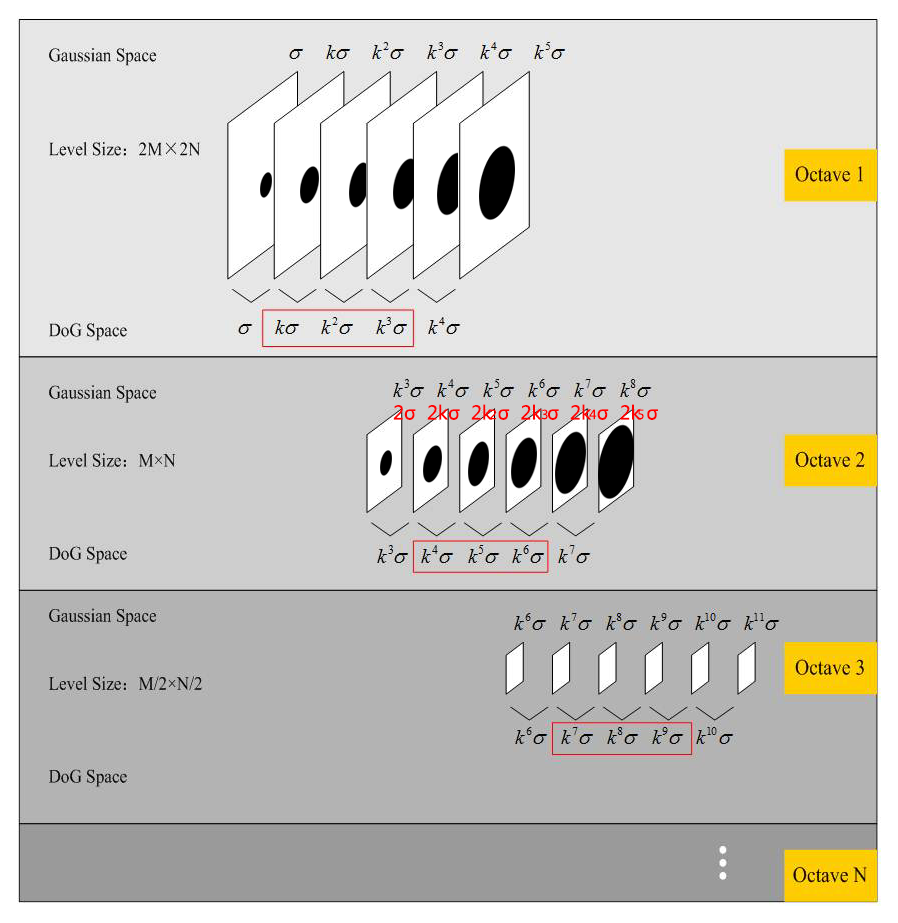
\includegraphics[width=14.00cm]{imgs/ch2/DoG}

图中的黑色圆盘是我加上去的,表示的是该图像所在的尺度的特征覆盖的范围,其特点是不同组同一层上的特征覆盖范围一样,同一组不同层上的特征覆盖范围逐步增大。关键点的尺度坐标就是按关键点所在的组和组内的层,利用下面这个公式计算而来:
\begin{equation}
  \sigma(o,s) = \sigma_0 2^{o+s/S},
  \quad o \in o_{\min} + [0, ..., O-1],
  \quad s \in [0,...,S-1]
\end{equation}

(2)SIFT检测子
sift算法有两个主要环节,一个是检测“感兴趣”的关键点,另一个是描述这个“关键点”。SIFT关键点是精心选择的一组在高斯差分尺度空间(Difference of Gaussians scale space,DoG)尺度空间上的极值点,该关键点包含三个关键信息,分别是(1)亚像素精度的(x,y)位置信息;(2)尺度大小,反映关键点局部的大小,同时决定了特征的覆盖范围,对后文局部块的提取起到至关重要的作用;(3)所在高斯尺度空间上的主方向,该主方向是有一个高斯窗口函数计算得来,反映的是关键点所在局部的方向信息。其中差分高斯尺度空间表示为
\begin{equation}
  D(x,\sigma(s,o)) \doteq G(x,\sigma(s+1,o)) - G(x,\sigma(s,o)).
\end{equation}

关于尺度空间和描述子的具体讲解在Lowe的论文中\cite{Lowe:2004uq}已有详细的介绍,这里不再详述。

(3)SIFT描述子
SIFT描述子反映关键点局部的信息,是高斯尺度空间上某一局部和方向上的梯度信息,以直方图的形式对信息做统计,最终每一个描述子是一个128的特征。


\section{图像配准}

先匹配,根据匹配的特征点对进行配准。

\subsection{2D几何变换}

(1)旋转和平移变换,也叫2D刚体运动即2D欧式变换(因其保持欧式距离),写作\(x={Rx+t}\)或者写作
\begin{equation}
	\begin{bmatrix}
	R & t
	\end{bmatrix}
	\bar{x}
\end{equation}
其中
\begin{equation}
	\begin{bmatrix}
	\cos{\theta} & -\sin{\theta} \\
	\sin{\theta} & \cos{\theta}
	\end{bmatrix}
\end{equation}
是一个正交旋转矩阵,有\(RR^T = I\)和\(|R| = 1\)

(2)放缩旋转,也叫做相似变换,该变换可以表示为\({\bar{x}}={sRx+t}\),其中s是一个任意的尺度因子。它也可以写作
\begin{equation}
	x ={ 
	\begin{bmatrix}
	sR & t
	\end{bmatrix}
	\bar{x}
	}
	={
	\begin{bmatrix}
	a & -b & t_x \\
	b & a & t_y
	\end{bmatrix}
	\bar{x}
	}
\end{equation}
其中我们不再需要\(a^2 + b^2 = 1\)。相似变换保持直线间的夹角。
各种2D变换如下表所示:
%![缩放](/img/posts/缩放.png)


\begin{table}[h]
\centering
\begin{tabular}{|c|c|c|c|}
\hline
\textbf{变换} & \textbf{矩阵大小} & \textbf{自由度数} & \textbf{保持} \\ \hline
平移          &   \(2\times{3}\)	& 2             & 方向          \\ \hline
刚性(欧式)    &   \(2\times{3}\) & 3             & 长度          \\ \hline
相似          &   \(2\times{3}\)  & 4             & 夹角          \\ \hline
仿射          &   \(2\times{3}\)  & 6             & 平行性         \\ \hline
投影          &   \(2\times{3}\)   & 8             & 直线性         \\ \hline
\end{tabular}
\caption{2D坐标变换}
\label{2dtrans}
\end{table}


当我们使用SIFT算法得到匹配到的特征点后,有两种方法,一种是直接写出变换矩阵,另一种是使用RANSAC方式多次迭代找到最准确的变换矩阵。RANSAC的方式将在后文介绍,我们先介绍根据一对匹配的SIFT算子直接写出两个图像块的变换矩阵。

结合一对匹配SIFT特征点\(\tilde{S}\)和\(S\)的位置、尺度和方向,我们可以得到两个图像块\(P_{\tilde{S}}\)和\(P_S\)的变换矩阵\(H_0\):

\begin{equation}
	H_0 = 
	\begin{bmatrix}
	\frac{\tilde{s}_f}{s_f} R & T
	\end{bmatrix}
\end{equation}
其中
\begin{equation}
	R = 
	\begin{bmatrix}
		\cos{(\tilde{\theta}-\theta)} & -\sin{(\tilde{\theta}-\theta)} \\
		\sin{(\tilde{\theta}-\theta)} & \cos{(\tilde{\theta}-\theta)} 
	\end{bmatrix}
\end{equation}

\begin{equation}
	T = 
	\begin{bmatrix}
		\tilde{x}_f - x_f \\
		\tilde{y}_f - y_f
	\end{bmatrix}
\end{equation}

计算出的\(H_0\)和\(H\)都可以作为块的旋转矩阵,在实际的系统中,我们会同时计算两个矩阵,比较他们的准确程度,挑选使用准确度高的变换矩阵。

\subsection{RanSAC}

\section{图像分割}

本文主要采用的是基于图的图像分割算法

\subsection{基于图的图像分割算法}

1、背景介绍

主要参考的是这篇文章《Efficient Graph-Based Image Segmentation》 Pedro F.Felzenszwalb

文章首先自己定义一种区域边界的度量方法,其度量方法是在基于图的图像表示法之上去定义的。
在这种度量方法之上,我们衍生出来比较高效的图像分割算法。该算法是一种贪婪算法,并且分割结果满足全局属性。

通过上述逻辑关系可以看出,文章定义的度量方法需要比较准确,有一定的物理意义在里面,不然即使算法再高效,度量本身有问题,那么分割出来的图像区域也是不准确的。那么文章自然的可以分为两个部分1)区域度量方法。2)高效分割算法

图像分割的在很多应用中非常重要,是很多高层应用的前提,比如识别、索引等,我们不具体举例。我们认为图像分割的方法有下面这样的特性:
\begin{itemize}
\item 能够捕捉到感知上比较重要的区域,这通常体现在图像的全局特性方面。这里有两个关键点,一方面要提供感知重要的精准属性,另一方面能够确定给定的分割技术是做什么的。我们认为应该有对分割结果属性的经确定以,这样的方法才能够更好的被理解,进而与其他的方法进行比较。
\item 高效,接近图像像素点数量的线性时间复杂度。为了能够实际使用,我们认为分割方法应该与边缘检测或者其他low-level图像处理技术有着相似的时间复杂度,意味着时间复杂度是线性,而且常系数也比较小。比如每一秒能对几帧图像进行分割的算法就能
够处理实时的视频数据。
\end{itemize}

然而,近几年的一些方法并不能够达成上述两方面要求,哪些方法太慢以致不能实践中使用。相比较而言,本文提到的方法已经因公在大尺度图像数据集应用上。有一些其他的方法可以比较快速的进行图像分割,但是这些方法不能捕捉感知上重要的非局部特性,下文会提到。总而言之,本文在保证效率的同时考虑到了图像全局属性上的感知重要区域。

首先我们来看一幅人造图像:

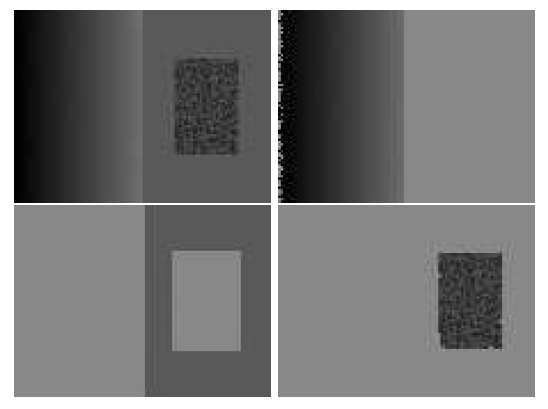
\includegraphics[width=15.00cm]{imgs/ch2/man_made}

我们人眼会认为这幅图像有三个区域,这个例子能够解释什么是感知重要属性(conceptually important property)。首先,亮度的变化不应该单独的座位分割区域的衡量标准。比如图像中左侧渐变区域和右侧的高频噪声区域都有较大的亮度变化,但是我们他们应该被分割成多个区域。因此,假设一个区域有着接近恒定的或变化很小的亮度是不正确的。

第二个感知重要属性是有意义的区域不能单纯的依靠局部划分标准。还是在图上我们可以看到原因,渐变图像与常量区域的边界上的亮度差值比很多高频区域的差值要小,因此我们得出结论,为了分割一幅图像,我们需要引入一些适应性的或者非局部的衡量标准。

我们在下一节提出的衡量标准会比较两个属性:
\begin{itemize}
\item 边界的亮度差值
\item 区域内部的邻居像素间的亮度差值
\end{itemize}
直观上,两个区域的边界上的亮度差值如果比比两个区域中至少一个区域的内部像素差值大的话,那么边界亮度差值会更多的影响我们的感知,这个时候我们说边界亮度差是感知重要的。

2、基于图的图像表示

好下面我们来进入正题,基于图的图像分割(Graph-Based Segmentation)。
我们使用基于图的方法来做图像分割,令\(G=(V,E)\)表示一个无向图,点集\(v_i \in V\),待分割的元素集合。边\((v_i,v_j) \in E\)有一个相应的权重\(w((v_i,v_j))\),是一个非负值,描述两个相邻元素\(v_i\)和\(v_j\)的不相似度。在图像分割,也就是本文的语境下,V中的元素就是像素点,边就是它的两个像素点(这两个像素点是相邻的)不相似性的某种度量(例如亮度,颜色,运动,位置或者其他局部属性)。在文章的最后我们会讨论比较特殊的边集合和权重函数,不过这里的公式和不相似性度量的方法是独立的,我们可以按照自己的需求定制度量方案,这里讨论的是大框架。

在基于图的方法中,一个分割方案S是V的一个划分,每一个区域(region or component)\(C \in S\)对应着图
\(G^` = (V,E^`)\)的一个连通区域,其中\(E^` \subseteq E\)。有许多方法来衡量一个分割的好坏,大体上我们希望\textbf{一个区域内部的元素尽可能相似,不同区域之间的像素尽可能不同}。这意味着同一区域内,相邻两个点的有相对来说比较小的权值,不同区域的相邻两个点的边有大的权值。

3、成对的区域比较预测,内部不相似度与外部不相似度

这一节我们首先定义一个预测,D,来估计是否存在一个显著的证据表明有一个边界能将两个区域分割开。就像上文说的,就是对外部的不相似性与内部不相似进行比较,也就是比较inter-component和within component的差值。

我们定义内部不相似性为该区域最小生成树的最大边,\(MST(C,E)\),即:
\begin{equation}
Int(C) = \mathop {\max }\limits_{e \in MST(C,E)}w(e)
\end{equation}

这个方法潜在的直觉是一个区域C,它保持连通的最低要求是Int(C)这个edge所决定的。

定义两个区域的不同:区域\(C_1,C_2 \subseteq V\),连接这两个区域的所有边的权值中,最小的那个权值。即,
\begin{equation}
Dif(C_1,C_2) = \mathop {\min }\limits_{v_i \in C_1 ,v_j \in C_2, (v_i,v_j) \in E}w((v_i,v_j))
\end{equation}

如果两个区域没有连接的边,则令\(Dif(C_1,C_2) = \infty\)
这个定义理论上可能会有问题,因为它只反映了(或者说只考虑到了)两个区域间权值最小的那条边。在实践中我们发现尽管有显著的局限,但这种度量方式结果颇佳。值得一提的是,改变这个衡量标准也是可以的,比如采用中位数或者其他的分位点,提升对异常值的鲁棒性,但这种改变会使问题编程NP-hard问题。因此一个小小的分割标准的改变会大大改变解决问题的难度。

区域比较预测法通过比较\(Dif(C_1,C_2)\)和\(Int(C_1)\)与\(Int(C_2)\)中较小的一个,来判断这两个区域是否有一个边界(换言之这两个区域是否有足够的理由保持两个区域)。

\begin{equation}
f(n) =\begin{cases} 
true,   \mbox {if } \mbox Dif(C_1,C_2) > M Int(C_1,C_2)\\\\
false,  otherwise \end{cases}
\end{equation}

我们引入了一个阈值函数来控制我们希望的外部不相似度与内部不相似度的相差程度。
\begin{equation}
MInt(C_1,C_2) = min(Int(C_1) + \tau(C_1),Int(C_2) + \tau(C_2))
\end{equation}
对于比较小的区域,\(Int(C)\)并不能够较好的反应局部特性,比如最极端的情况下,当\(|C| = 1\)时,\(Int(C) = 0\)。因此我们需要一个跟区域大小相关的阈值函数
\[\tau (C) = \frac{k}{|C|}\]
其中\(|C|\)表示的是区域C的大小,k是一个常数。越是小的区域,我们越希望较大的外部不相似性。
在实际中,我们可以调整k的取整来获得不同的效果。当k值很大时,算法倾向于分割出来较大的块,当k值较小时,算法倾向于更细的划分。

本节最后我们探讨一个比较有趣的话题,就是\(\tau\)函数的选取,如果我们改变这个函数,不会对算法的大框架造成影响,而会对分割结果的倾向性有影响。比如我们可以让分割倾向于某一种形状A,令\(\tau\)函数在区域不是形状A的时候较大即可。这种形状上的倾向可以比较简单,比如希望正方形的或者扁平状的,也可以比较复杂,是一种特殊的形状。

4、分割算法

本节讲解主要的算法部分,怎样利用上述的定义,在基于图的表示方法下,做出高效而准确的分割。算法的核心:

输入是一个图\(G=(V,E)\),有n个点和m个边。输出是一个分割V,分割成\(S=(C_1,...,C_2).\)

\begin{enumerate}
\item 对E进行排序,生成非递减的序列\(\pi = (o_1,...,o_m)\)
\item 从初始分割\(S^0\)开始,每一个点\(v_i\)自己就是一个区域
\item 对于每一个\(q = 1,...,m\)重复步骤3
\item 通过\(S^{q-1}\)构建\(S^q\),使用如下的方式:令\(v_i\)和\(v_j\)表示按顺序排列的第q条边的两个点,比如\(o_q = (v_i,v_j)\)。如果\(v_i\)和\(v_j\)在\(S^{q-1}\)中连个不同的区域下,并且\(w(o_q)\)比两个区域的内部不相似度都小,那么合并这连个区域,否则什么也不做。用公式来表达就是:令\(C_{i}^{q-1}\)是\(S^{q-1}\)的一个区域,它包含点\(v_i\);令\(C_{j}^{q-1}\)是\(S^{q-1}\)的一个区域,它包含点\(v_j\)。如果\(C_{i}^{q-1} \neq C_{j}^{q-1}\)并且\(w(o_q) \leq MInt(C_i^{q-1},C_j^{q-1})\),那么通过合并\(C_{i}^{q-1}\)和\(C_{j}^{q-1}\)我们得到了\(S^q\);否则的话\(S^q = S^{q-1}\)
\item 返回\(S = S^m\)
\end{enumerate}

分割结果如图所示:

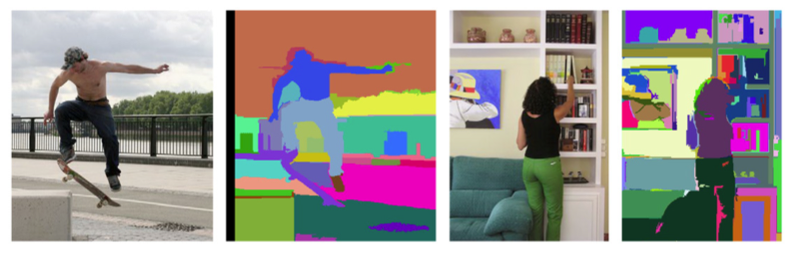
\includegraphics[width=15.00cm]{imgs/ch2/segment}

\section{图像融合}

%% 本章参考文献
\ifx\usechapbib\empty
\nocite{BSTcontrol}
\bibliographystyle{buptgraduatethesis}
\bibliography{bare_thesis}
\fi